% Full draft for a conference / journal submission — generic template (plain article class). To move to a venue class
% (IEEEtran, acmart, llncs, ...), keep the body and replace the preamble and the front matter.
% Build:  latexmk -pdf main.tex
% Figures: figures/paper_figures.ipynb (style: figures/paper_style.py; dataset_construction.py runs on the server)
% Notes for the authors would be in \todo{...} (red). The previous draft is in _da_cancellare/.
\documentclass[11pt,a4paper]{article}
\usepackage[margin=2.5cm]{geometry}
\usepackage[T1]{fontenc}
\usepackage[utf8]{inputenc}
\usepackage{lmodern}
\usepackage{amsmath,amssymb}
\newcommand{\Y}{\checkmark}
\newcommand{\N}{$\times$}
\usepackage{graphicx}
\usepackage{booktabs}
\usepackage{xcolor}
\usepackage{tikz}
\usetikzlibrary{arrows.meta,positioning,shapes.misc}
\usepackage[numbers,sort&compress]{natbib}
\usepackage[colorlinks=true,linkcolor=blue!50!black,citecolor=blue!50!black,urlcolor=blue!50!black]{hyperref}
\def\UrlBreaks{\do\/\do-\do\_\do.}
\usepackage{authblk}
\usepackage{orcidlink}
\renewcommand\Affilfont{\small}

\newcommand{\todo}[1]{\textcolor{red}{[\textbf{TODO:} #1]}}
\newcommand{\anon}{\operatorname{anon}}

\title{Traces of Reliability: What the Anonymized Articles of Unseen News Publishers Reveal about Their Rating, and How
Leakage Inflates It}
\author[1]{John Bianchi\,\orcidlink{0009-0006-2582-1480}\thanks{Corresponding author: John Bianchi
(\texttt{john.bianchi@imtlucca.it}).}}
\author[2]{Manuel Pratelli\,\orcidlink{0000-0002-9978-791X}}
\author[1]{Fabio Pinelli\,\orcidlink{0000-0003-1058-6917}}
\author[2,1]{Marinella Petrocchi\,\orcidlink{0000-0003-0591-877X}}
\affil[1]{IMT School for Advanced Studies Lucca, 55100 Lucca, Italy\\
\texttt{\{john.bianchi, fabio.pinelli\}@imtlucca.it}}
\affil[2]{Institute of Informatics and Telematics, National Research Council (IIT-CNR), 56124 Pisa, Italy\\
\texttt{\{manuel.pratelli, marinella.petrocchi\}@iit.cnr.it}}
\date{}

\begin{document}
\maketitle

\begin{abstract}
Professional raters such as NewsGuard rate news outlets one by one, and many outlets remain unrated. We ask whether the
rating of an unseen outlet can be predicted from the text of its articles once everything that names the outlet has
been removed, and how much weaker evaluation protocols inflate the results. To our knowledge, no previous study keeps the outlets of the same owner apart. On 25,524 articles from 226 English-language political outlets rated by NewsGuard, we keep the
test outlets and their owners out of training, remove articles copied across outlets, and mask links, e-mail addresses
and the names of outlets and journalists. A model scores each article; the score of an outlet is the mean over its
articles. The best model is a ridge regression on the hidden states of the frozen Mistral-Small-24B. Its mean absolute
error on the NewsGuard scale (0--100) is 15.8 points, against 17.8 for TF-IDF and 22.1 for a constant; it ranks the
outlets with a Spearman correlation of 0.74 and separates reliable from unreliable ones with an AUC of 0.88. Its error
is lower than that of TF-IDF in every condition we tested, most of all with few articles: with one article per outlet
it is 17.3 points against 20.5. Small encoders do not beat TF-IDF. Weaker protocols inflate the results: splitting
articles instead of outlets, or training on sister sites of the same owner, lowers the error by 6--12 points, while
masking the names changes it by less than half a point. These
models can help raters to decide which unrated outlets to examine first. We release the code, the models, the
predictions and a local tool.
\end{abstract}

\noindent\textbf{Keywords:} news source reliability; evaluation protocol; data leakage; anonymization; media
profiling; large language models; NewsGuard.

% =====================================================================================================================
\section{Introduction}\label{sec:intro}

In contemporary digital media ecosystems, assessing the reliability of news publishers has become an important means
of limiting the spread of misleading or low-quality information~\cite{Bowman2003,Jemielniak2020}. Organizations such as
NewsGuard, the Global Disinformation Index and Media Bias/Fact Check rate news outlets on journalistic standards such as
transparency, editorial accountability, factual accuracy and corrections, and their ratings largely
agree~\cite{lin2023high,DBLP:conf/icwsm/PratelliP22}. Each rating is made by trained journalists, outlet by outlet, so
many outlets, especially new and small ones, remain unrated for a long time.

Automatic methods could help. Many predict credibility from articles~\cite{pandolfi2020automatic,Przybyla2021plugin,
10.1145/3770077,DBLP:journals/dbsk/AdjiLS26} or profile media sources from their articles and other
signals~\cite{baly2018predicting,baly2020written,nakov2024survey}. When the labels come from ratings of publishers,
however, two problems can make the results look better than they are. First, if the same publisher is in the training
and in the test data, a model can learn to recognize the publisher instead of learning what makes it
reliable~\cite{zhou2021hidden,azizov-etal-2024-safari,verhoeven2025yesterday}. Second, even with different publishers
in training and test, the text often reveals its source: the outlet's name, the names of its journalists, the links to
its own pages and, as we show in Section~\ref{sec:groups}, whole articles copied across sites of the same owner. In both
cases a model can recognize an outlet without judging its writing. In previous work we classified articles into the reliability levels of their publishers and aggregated them into a
level per publisher, on publishers never seen in training~\cite{Bianchi2024SAC,bianchi2026articles}. Here we remove both problems.

Our question is how much of a professional rating the anonymized text of an outlet still carries once these
shortcuts are removed, and how much the shortcuts inflate the results when they are left in place. The answer is not
obvious, because NewsGuard checks its criteria outside the articles, for instance by verifying claims against other
sources or by reading the \emph{about} page of an outlet for its ownership and financing. Still, the way an outlet works
may leave traces in how it writes: how it sources and hedges claims, whether it separates news from opinion, which
topics it covers and in what tone. We look for these traces, and not for the identity of the outlet.

We treat the problem as a regression at the level of the publisher. A model predicts a score for each article, and the
score of a publisher is the mean of the predictions for its articles, so the judgment on an outlet always rests on
several articles. The evaluation follows four rules: the test outlets never appear in training, outlets of the same
owner are never split between training and test, articles copied across outlets are removed, and every article is
anonymized before any model reads it. Within these rules we compare models from TF-IDF to large language models. Our
contributions are:
\begin{enumerate}
  \item \textbf{A protocol, a dataset and a measure of leakage.} Outlet-disjoint splits with ownership groups,
        deduplication across outlets and anonymization, applied to 25,524 articles from 226 political outlets. Without
        these protections the error falls by 6--12 points, while masking the names changes it little
        (Sections~\ref{sec:data} and~\ref{sec:ladder}).
  \item \textbf{A comparison of models.} Large frozen language models with a linear head beat TF-IDF in every condition
        we tested, most of all with few articles per outlet; small encoders and zero-shot prompting do not
        (Sections~\ref{sec:stage1}, \ref{sec:stage2} and~\ref{sec:k}).
  \item \textbf{An analysis of the errors} by reliability level (Section~\ref{sec:errors}).
  \item \textbf{Open resources:} the code, the models, the predictions and a local tool (Section~\ref{sec:tool}).
\end{enumerate}

% =====================================================================================================================
\section{Related Work}\label{sec:related}

\paragraph{Publisher reliability.} Credibility is often assessed article by article~\cite{pandolfi2020automatic,
10.1145/3770077}, but the reputation of the source strongly shapes how information is
perceived~\cite{doi:10.1080/07421222.2019.1628921}. The ratings of NewsGuard, the Global Disinformation Index and Media
Bias/Fact Check (MBFC) largely agree and are widely used as ground truth~\cite{lin2023high,DBLP:conf/icwsm/PratelliP22}.
The reliability of a publisher has been predicted from writing style~\cite{przybyla2020capturing,potthast2018stylometric},
from user interactions, social networks, web graphs and
metadata~\cite{bazmi2023multi,DBLP:conf/ecir/PratelliSP25,DBLP:conf/icwsm/WilliamsCC25,DBLP:journals/jdiq/LongoZCZC25},
and from articles combined with Wikipedia, social media and audience
data~\cite{baly2018predicting,baly2020written,nakov2024survey}. Large language models have also been asked to rate named
sources~\cite{yang2023large} or to produce weak credibility labels~\cite{Leite2025}. Given the name of a source, however,
a model may simply recall what it knows about it, which is why we mask the names.

\paragraph{Evaluation on unseen sources.} Zhou et al.~\cite{zhou2021hidden} showed that models trained on labels
inherited from the sources learn the sources themselves, and that random splits of the articles overestimate
performance. Later work found that performance drops under shifts of domain, time and
publisher~\cite{azizov-etal-2024-safari,burdisso-etal-2024-reliability,verhoeven2025yesterday}. Table~\ref{tab:related}
compares the studies closest to ours, which predict reliability mainly from text with labels given to the sources. All
those that compare seen with unseen sources report a drop: from 0.91 to 0.65 F1 in Rashkin et
al.~\cite{rashkin2017truth}, from 0.94 to 0.86 AUC in Horne et al.~\cite{horne2019robust}, from 0.998 to 0.796 accuracy
in Przyby{\l}a~\cite{przybyla2020capturing}, from 0.97 to 0.72 AUC in Bozarth and Budak~\cite{bozarth2020toward}, from 0.92 to 0.73
accuracy for BERT in Huang et al.~\cite{huang2020conquering} and from 0.97 to 0.80 accuracy in Zhou et
al.~\cite{zhou2021hidden}.
None of them keeps the outlets of the same owner apart, although outlets often share
content~\cite{horne2019spirals,gruppi2021tell}. Huang et al.\ remove the sources that copy reliable outlets, and
Verhoeven et al.\ remove duplicated titles and URLs across their dataset, and Manzoor et al.~\cite{manzoor2026multiview}
keep articles on the same story on one side of the split; Bozarth and Budak and Verhoeven et al.\ mask the names of
outlets. All of them except Kondrup et al.~\cite{kondrup2026credibench} predict classes. Continuous reliability has been estimated from the links between news
sites~\cite{burdisso-etal-2024-reliability} and from the web graph, the text and time~\cite{kondrup2026credibench}, and
Eldifrawi et al.~\cite{eldifrawi2026temporal} classify the credibility of domains, without their names, from the
judgments of a language model on their articles, with evidence from web search, aggregated by a decision tree. We measure how much of the full 0--100 score the anonymized text alone carries under all the protections above,
and what each protection changes. Datasets with source-level labels include NELA-GT~\cite{gruppi2021nela} and the BAT corpus~\cite{DBLP:journals/dbsk/AdjiLS26,batDataset}, and splits by publisher were already used in the hyperpartisan
task of SemEval-2019~\cite{kiesel2019semeval}.

\begin{table}[t]
\centering\small
\caption{Comparison with the closest studies, in chronological order. Each row is a study and each column a property of
its setting: what the model reads (\emph{other}: Wikipedia, social media, URL and traffic for Baly et al., backlinks and
page design for Eldifrawi et al., graphs of audience, links and similarity for Manzoor et al.; \emph{links}: a separate
model on the links between domains; \emph{web graph}: the links between domains, read with the text; \emph{network}: a network
of content shared between sources), where the labels come from, whether the test sources are absent from training
(\emph{in part}: in one experiment), whether outlets of the same owner are kept on the same side of the split, whether
articles copied across outlets are removed before the split (\emph{in part}: only some sources or some kinds of copies;
\emph{unclear}: duplicates removed, scope not stated), which names are removed from the text (\emph{all}: outlets,
journalists, links and e-mail addresses), and what is predicted ($^\ast$: hyperpartisan, not reliability; DQR: the aggregate ratings of Lin et
al.~\cite{lin2023high}). --: not done or not reported.}\label{tab:related}
\footnotesize\setlength{\tabcolsep}{3pt}
\resizebox{\linewidth}{!}{%
\begin{tabular}{llllllll}
\toprule
study & input & labels & unseen & owners & copies & names & target \\
 & & & sources & apart & removed & masked & \\
\midrule
Rashkin et al.~\cite{rashkin2017truth} & text & source type & yes & -- & -- & -- & 4 classes per article \\
Baly et al.~\cite{baly2018predicting} & text + other & MBFC & yes & -- & -- & -- & 3 classes per source \\
Fairbanks et al.~\cite{fairbanks2018credibility} & text; links & MBFC & -- & -- & -- & -- & 2 classes per article \\
Horne et al.~\cite{horne2019robust} & text + Wikipedia & NewsGuard, OpenSources & in part & -- & -- & -- & 2 classes per article \\
Kiesel et al.~\cite{kiesel2019semeval} & text & BuzzFeed, MBFC & yes & -- & -- & links & 2 classes per article$^\ast$ \\
Przyby{\l}a~\cite{przybyla2020capturing} & text & PolitiFact, Pew & in part & -- & unclear & -- & 2 classes per article \\
Bozarth \& Budak~\cite{bozarth2020toward} & text or social & MBFC & in part & -- & -- & outlets & 2 classes per article \\
Huang et al.~\cite{huang2020conquering} & text & NELA-GT & in part & -- & in part & -- & 2 classes per article \\
Baly et al.~\cite{baly2020written} & text + other & MBFC & yes & -- & -- & -- & 3 classes per source \\
Zhou et al.~\cite{zhou2021hidden} & text & MBFC & in part & -- & -- & -- & 2 classes per article \\
Gruppi et al.~\cite{gruppi2021tell} & text + network & NewsGuard, OpenSources & yes & -- & -- & -- & 2 classes per article \\
Azizov et al.~\cite{azizov-etal-2024-safari} & text & MBFC & yes & -- & unclear & -- & factuality levels per source \\
Bianchi et al.~\cite{bianchi2026articles} & text & NewsGuard & yes & -- & -- & -- & 5 classes per source \\
Eldifrawi et al.~\cite{eldifrawi2026temporal} & text + search + other & MBFC & yes & -- & unclear & -- & 3 classes per source \\
Verhoeven et al.~\cite{verhoeven2025yesterday} & text & MBFC & in part & -- & yes & own outlet, links & 2 classes per article \\
Kondrup et al.~\cite{kondrup2026credibench} & text + web graph & DQR & yes & -- & -- & -- & score per source \\
Manzoor et al.~\cite{manzoor2026multiview} & text + other & MBFC & yes & -- & in part & -- & 3 or 5 classes per source \\
\midrule
this work & text & NewsGuard & yes & yes & yes & all & score 0--100 per source \\
\bottomrule
\end{tabular}}
\end{table}

\paragraph{Models and anonymization.} Fine-tuned encoders such as BERT and
ModernBERT~\cite{devlin2019bert,warner2024modernbert} are the usual choice for text classification and regression. When
the independent training units are few, a common alternative is to keep a large pretrained model frozen and to train only
a linear model on its representations, taken from embedding models that follow an instruction~\cite{zhang2025qwen3} or
from the intermediate layers of decoder models~\cite{skean2025layer}. To mask outlets and journalists we use
GLiNER~\cite{zaratiana2024gliner}, a zero-shot named-entity recognizer that accepts entity types described in natural
language.

% =====================================================================================================================
\section{Problem Definition and Methodology}\label{sec:problem}

\subsection{Problem definition}\label{sec:definition}
Let $A$ be a corpus of news articles, each with a text $t_a$ and a publisher $p(a) \in P$, and let $A_p$ be the articles
of publisher $p$. Each publisher has a NewsGuard score $s(p) \in [0, 100]$ (Section~\ref{sec:labels}). There are no
labels for single articles, so every article inherits the score of its publisher. Before any model reads an article, a function $\anon$ replaces the names of
outlets and journalists, the links and the e-mail addresses with placeholders (Section~\ref{sec:anon}).

\paragraph{Stage 1: articles.} A regressor $f$ predicts the score of each article, $\hat{s}(a) = f(\anon(t_a))$.

\paragraph{Stage 2: publishers.} The score of a publisher is the mean of the predictions for its articles,
$\hat{s}(p) = \frac{1}{|A_p|} \sum_{a \in A_p} \hat{s}(a)$. All the results of the paper are computed on these
publisher scores, except those of Section~\ref{sec:stage1}, and Section~\ref{sec:k} varies the number of articles used.

\paragraph{Separate publishers and owners.} Since all the articles of a publisher share its score, the split is made over
publishers, so that the training and test publishers are disjoint,
\begin{equation}\label{eq:disjoint}
P_{\text{train}} \cap P_{\text{test}} = \emptyset .
\end{equation}
Publishers of the same owner may publish the same articles under different names. We therefore also keep one publisher
per ownership group $g(p)$ (Section~\ref{sec:groups}), so that $g(p) \neq g(q)$ for every $p \in P_{\text{train}}$ and
$q \in P_{\text{test}}$, and we remove duplicated articles across publishers.

\subsection{Evaluation metrics and baselines}\label{sec:metrics}
Every metric compares the predicted score of each test publisher, that is the mean of the predictions for its
articles, with its NewsGuard score. Only Section~\ref{sec:stage1} applies the same metrics to single articles.

\paragraph{Error.} The main metric is the mean absolute error, $\mathrm{MAE} = \frac{1}{|P|} \sum_{p} |\hat{s}(p) -
s(p)|$, in NewsGuard points: how far, on average, a prediction is from the rating. We also report the share of
publishers predicted within 20 points of their score, the width of the second NewsGuard level (40--59).

\paragraph{Ranking.} To rank outlets, for instance to decide which unrated outlets to review first, the order of the
predictions matters more than their values. We report Spearman's $\rho$ and Kendall's $\tau_b$, which handles ties (the
226 outlets have only 45 distinct scores). Appendix~\ref{app:measures} adds $R^2$, the root mean squared
error and the AUC for separating reliable outlets (score $\geq 60$) from the others.

\paragraph{Baselines.} TF-IDF with a ridge regression (Section~\ref{sec:setup}) is the reference text model: every
language model is compared with it. Two further baselines use no text:
\begin{itemize}
  \item \textbf{Training median:} the best constant prediction for the MAE, computed on the training publishers.
  \item \textbf{Training mean:} the best constant prediction for the squared error.
\end{itemize}

\paragraph{Statistical testing.} Intervals are 95\% bootstrap intervals over publishers~\cite{efron1979bootstrap}. Two
models are compared on the same bootstrap resamples, and the $p$-values are corrected for multiple comparisons with the
Holm method~\cite{holm1979simple} (Appendix~\ref{app:stats}). We call a difference significant when it
remains so after the correction, at the 5\% level.

% =====================================================================================================================
\section{Dataset}\label{sec:data}

\subsection{Ground truth: NewsGuard}\label{sec:labels}
In NewsGuard~\cite{newsguard}, trained journalists rate online news outlets on nine criteria, which include whether an
outlet repeatedly publishes false content, corrects its errors, separates news from opinion, avoids deceptive headlines
and discloses its ownership and financing. The score $s(p)$ is the weighted sum of the criteria met. NewsGuard also
groups the score in five levels, 0--39 ($l_1$), 40--59 ($l_2$), 60--74 ($l_3$), 75--99 ($l_4$) and 100 ($l_5$), which we
use to describe the data. We use the ratings of 23 October 2026 (76\% of them updated in 2025 or 2026) for the outlets
whose only topic is \emph{political news or commentary}. The ratings are licensed and cannot be redistributed. They
largely agree with those of other raters~\cite{lin2023high}. We use the ratings as the target of the
task.

\subsection{Collection and cleaning}\label{sec:cleaning}
In October 2026 we collected about 200 recent articles from the website of each political outlet rated by NewsGuard,
saving the raw HTML. The collector follows feeds, sitemaps and homepage links, respects robots.txt and makes at most one
request per second to each site. Of the 1,293 outlets, 674 returned at least one article; the others were offline,
blocked automated access or had no article pages. Table~\ref{tab:cleaning} lists the filters, applied in this order:
\begin{itemize}
  \item \textbf{Text extraction:} trafilatura~\cite{barbaresi2021trafilatura} in precision mode keeps the main text of
        each page.
  \item \textbf{English}, detected with langdetect on the first 400 words.
  \item \textbf{100--1,500 words}, to drop short notices and very long pages such as transcripts and live blogs.
  \item \textbf{Published from 2025.}
  \item \textbf{No duplicates across outlets:} exact copies and near copies (Jaccard similarity of word 5-grams of at
        least 0.5, estimated with MinHash~\cite{broder1997resemblance}) are removed across all outlets, keeping the
        oldest. Removing them only within each outlet would leave the same article in training and test under two
        different outlets.
  \item \textbf{At least 10 articles} per outlet.
  \item \textbf{One outlet per ownership group}, the one with the most articles (Section~\ref{sec:groups}).
\end{itemize}

\begin{table}[t]
\centering
\caption{Dataset construction. Each row is a filter, applied in order from top to bottom; the columns give the articles
and the outlets left after it. The last row is the final dataset.}\label{tab:cleaning}
\begin{tabular}{lrr}
\toprule
step & articles & outlets \\
\midrule
political outlets with at least one article & 86,225 & 674 \\
text extracted from the HTML & 85,303 & 668 \\
English & 67,231 & 577 \\
100--1,500 words & 52,027 & 565 \\
published from 2025 & 40,232 & 531 \\
no exact duplicates & 34,799 & 361 \\
no near duplicates (Jaccard $\geq 0.5$) & 33,694 & 347 \\
at least 10 articles per outlet & 33,443 & 287 \\
one outlet per ownership group & \textbf{25,524} & \textbf{226} \\
\bottomrule
\end{tabular}
\end{table}

\subsection{Ownership groups and shared text}\label{sec:groups}
Outlets of the same owner often publish the same articles under different names~\cite{horne2019spirals}, and a model
trained on one of them could recognize the others in the test set. We link two outlets if NewsGuard gives them the same
owner (ignoring legal forms such as \emph{Inc}) or the same parent domain, and we call the connected sets
\emph{ownership groups}. The 1,293 political outlets form 589 groups. In these groups 797 outlets have at least one
\emph{sister}, and keeping one outlet per group removes 704 of them. Most sisters already disappear with deduplication,
because the sites of a network publish the same texts and only the oldest copy is kept (Figure~\ref{fig:groups}); the
last filter removes the remaining 61.

\begin{figure}[t]
\centering
\includegraphics[width=\linewidth]{figures/groups.pdf}
\caption{Outlets through the cleaning. Each bar is a filter of Table~\ref{tab:cleaning}; the bar is split between the
outlets kept for their ownership group (hatched \texttt{//}) and their sister outlets (hatched
\texttt{\textbackslash\textbackslash}); the number of articles is in parentheses.}\label{fig:groups}
\end{figure}

Figure~\ref{fig:network} places every outlet on a two-dimensional map of its texts and follows it through the
cleaning. Outlets of the same large network cluster tightly, since they publish the same articles: the largest
ownership group, 164 sites all in the lowest level, is the dense cluster that deduplication almost entirely removes,
because afterwards none of its sites keeps 10 articles. Before deduplication, 19.4\% of the articles have a copy
(Jaccard similarity of word 5-grams $\geq 0.5$) in an outlet of the same owner and 2.7\% in an outlet of another owner,
and 98\% of the pairs of outlets that share articles have the same owner (Appendix~\ref{app:sisters}). Without these
filters, the network of 164 sites would sit on both sides of every split, and a model could score its test sites by
recognizing copies of its training sites. Sisters are similar even without copies: after deduplication, 59\% of the 81
outlets that still have a sister are closer, in TF-IDF similarity, to a sister than to any outlet of another group, and
sisters usually share their rating (Appendix~\ref{app:sisters}). Section~\ref{sec:ladder} measures what keeping them
would change.

\begin{figure}[t]
\centering
\includegraphics[width=\linewidth]{figures/group_maps.pdf}
\caption{Ownership groups through the cleaning. Each panel is a cleaning step of Table~\ref{tab:cleaning}. Every outlet
with extracted text sits at the same place on a two-dimensional map of its texts (t-SNE of the mean TF-IDF vector of its
articles, with the outlet's own name, links and e-mail addresses removed; nearby outlets write alike); only the outlets
that survive the step are drawn, the others as a grey trace. The three largest ownership groups, as recorded before cleaning, have their own marker, the outlets of the
smaller groups (2--15 outlets) share another one, and the outlets without sisters are grey. The number of sisters is the number of outlets minus the number of distinct ownership groups still present: the
last panel keeps one outlet per group, so it has none, and the dense cluster of the 164-site network is gone.}\label{fig:network}
\end{figure}

\subsection{Anonymization}\label{sec:anon}
A model could recognize an outlet from its name, its journalists or its links. The function $\anon$ replaces them with placeholders,
without rewriting the text, in two stages:
\begin{itemize}
  \item \textbf{Rules:} regular expressions replace links and e-mail addresses with \texttt{[URL]} and \texttt{[EMAIL]},
        and the name of the publishing outlet, derived from its domain, with \texttt{[OUTLET]};
  \item \textbf{GLiNER:} GLiNER~\cite{zaratiana2024gliner}, a zero-shot named-entity recognizer, then replaces the names
        of all news outlets, the publishing outlet included, with \texttt{[OUTLET]} and the names of all journalists
        with \texttt{[AUTHOR]}.
\end{itemize}
The rules make sure that the most direct trace, the outlet's own name, is removed; GLiNER extends the masking to every
outlet and journalist. Section~\ref{sec:ladder} compares this anonymization with the rules alone.
Every outlet and journalist is masked, including those other than the publisher, because citing other outlets can
reveal the position of an outlet among them, and because the recognizer cannot tell the outlet's own staff from other
journalists. After anonymization, the name of the publishing outlet remains in 1.6\% of the articles (37.8\%
before), mostly where the name is also a common word. The brand name recorded by NewsGuard remains in 2.1\% of the
articles, concentrated in 17 outlets, and social-media handles in 9.5\%. Appendix~\ref{app:anonfig} gives the settings and the counts of each step. The placeholders keep a trace of how an outlet writes, such as whether it
cites sources and signs its articles, but not of which outlet it is. We do not remove style, topics or political stance,
since they are the signal we study.

\subsection{The final dataset}\label{sec:final}
The dataset has 25,524 articles from 226 outlets, with a median of 112 articles per outlet (from 10 to 201;
Figure~\ref{fig:dataset}). Scores lean towards reliable outlets (median 75, Figure~\ref{fig:dataset}a): 35 outlets are in the lowest level, 43 in
40--59, 30 in 60--74, 79 in 75--99 and 39 have a perfect score. No article exceeds the input length of any model (median
about 760 tokens, at most about 3,000).

\paragraph{Representativeness.} The dataset is not a random sample of the rated outlets. We set filters on the
text and on the ownership, never on the score, but they remove many low scores: 15\% of the dataset is in the lowest
level, against 33\% of all the outlets rated by NewsGuard, mostly because 619 outlets returned no article (mean score
41), and cannot be scored from their text by any method, and 170 published only copies (mean 37). These are also the
outlets on which the models err most (Section~\ref{sec:errors}): the test has fewer of the hardest cases, and the
training fewer examples of them. Appendix~\ref{app:selection} compares the dataset with NewsGuard and discusses both
effects.

\begin{figure}[t]
\centering
\includegraphics[width=\linewidth]{figures/dataset.pdf}
\caption{The final dataset. (a) Number of outlets in each NewsGuard level; (b) number of articles of each outlet, with the outlets
sorted from the fewest to the most articles (at least 10); (c) NewsGuard scores of the outlets in each of the five
folds.}\label{fig:dataset}
\end{figure}

% =====================================================================================================================
\section{Experiments}\label{sec:experiments}

\begin{figure}[t]
\centering
\resizebox{\linewidth}{!}{%
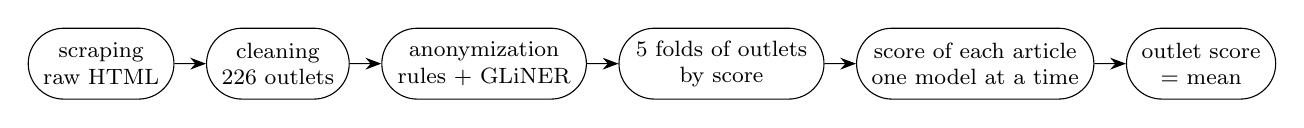
\begin{tikzpicture}[node distance=4mm, box/.style={draw, rounded rectangle, align=center, font=\footnotesize,
  minimum height=9mm, inner sep=3pt}, >={Stealth[length=2mm]}]
\node[box] (s) {scraping\\raw HTML};
\node[box, right=of s] (c) {cleaning\\226 outlets};
\node[box, right=of c] (a) {anonymization\\rules + GLiNER};
\node[box, right=of a] (f) {5 folds of outlets\\by score};
\node[box, right=of f] (m) {score of each article\\one model at a time};
\node[box, right=of m] (o) {outlet score\\= mean};
\foreach \x/\y in {s/c, c/a, a/f, f/m, m/o} \draw[->] (\x) -- (\y);
\end{tikzpicture}}
\caption{The pipeline. Each box is a step, from the collected pages (left) to the score of each outlet
(right).}\label{fig:pipeline}
\end{figure}

\subsection{Experimental setup}\label{sec:setup}
We use a 5-fold cross-validation over outlets (Figure~\ref{fig:pipeline}). The outlets are sorted by score and, in
blocks of five, assigned at random to different folds, so that every fold has the same score distribution
(Figure~\ref{fig:dataset}c). Each model is trained on four folds (about 180 outlets and 20,000 articles) and tested on
the fifth, so every outlet is scored once by a model that never saw it. The settings of the linear models (the ridge
penalty and, for Mistral-Small-24B, the layer) are chosen on three inner folds of the training outlets. In training every
article counts once, while in the evaluation every outlet counts once. The models read the body of each article, not the
title. We compare:
\begin{itemize}
  \item \textbf{TF-IDF + ridge:} word uni- and bi-grams with a ridge regression~\cite{hoerl1970ridge}, the standard
        strong baseline for vocabulary, topic and style.
  \item \textbf{Frozen language models + ridge:} a pretrained model, not trained on our data, turns each article into a
        vector, and a ridge regression on these vectors is the only part trained on the scores. We use the embedding
        models Qwen3-Embedding-8B and Qwen3-Embedding-0.6B~\cite{zhang2025qwen3}, given an instruction to represent the
        article for judging the reliability of its outlet; the base decoder Mistral-Small-24B~\cite{mistralsmall} in
        4-bit quantization~\cite{dettmers2023qlora}, through the mean hidden state of an intermediate
        layer~\cite{skean2025layer} (layer 27, chosen on the inner folds); and ModernBERT-base without training.
  \item \textbf{ModernBERT, fine-tuned:} the 150-million-parameter encoder~\cite{warner2024modernbert} trained end to end
        on the scores.
  \item \textbf{Mistral-Small-24B-Instruct, zero-shot:} the instruction-tuned Mistral is asked for the NewsGuard score of
        the site that published each article, with a prompt that describes the nine criteria (Appendix~\ref{app:prompt}).
\end{itemize}
The two Qwen3 models differ in size, the two ModernBERT models only in their training, and the two Mistral models in how
they use the text. Appendix~\ref{app:impl} gives all the settings. Every random choice is seeded, and the predictions and the models of
every fold are saved.

\paragraph{Development on the same outlets.} The rules of the dataset, the split and the models were fixed after earlier
rounds of experiments on the same 226 outlets, whose test results we saw (Appendix~\ref{app:tried}); only the ridge
penalty and the Mistral layer are chosen inside the training folds. Part of the differences between models could
therefore reflect an adaptation of the design to these outlets. Three facts limit this risk, without removing it. First,
the rules are fixed thresholds that we did not tune (100--1,500 words, from 2025, at least 10 articles), and the frozen
models are used without any adaptation, with the plainest head, a ridge regression: fourteen other regressors tried on
the same outlets were not much better. Second, the one design choice that we could run again end to end, the
anonymization, changes the error of every model by less than half a point (Appendix~\ref{app:anon}). Third, the gap
between Mistral-Small-24B and TF-IDF is 2.0--2.3 points in each of five splits of the outlets, and the split of the paper
is the one in which it is smallest (Appendix~\ref{app:splits}). None of this replaces a test on new outlets. The
released frozen models can be applied to them without any change (Section~\ref{sec:tool}), and the effects of the protocol (Section~\ref{sec:ladder}), several times larger than the differences between models,
are much less exposed to this risk.

\subsection{Stage 1: article-level score estimation}\label{sec:stage1}
Table~\ref{tab:article} compares each test article with the score of its outlet. All models do better than chance, and
Mistral-Small-24B is the best (MAE 17.8, $\rho = 0.61$). A single article, however, is a weak signal: the trained models
put it within 20 points of the score of its outlet in 54--64\% of the cases, against 50\% without text. This is
expected, since every article inherits the score of its outlet, while a reliable outlet can publish a weak opinion piece
and an unreliable one a plain factual report. For this reason we judge each outlet on several articles.

\begin{table}[t]
\centering
\caption{Stage 1, single articles. Each row is a model; each of the 25,524 test articles is compared with the NewsGuard
score of its outlet. Lower MAE and higher $\rho$ and share within 20 points are better; the best value is in bold. The
rows above the line are baselines.}\label{tab:article}
\begin{tabular}{lccc}
\toprule
model & MAE (points) & Spearman $\rho$ & within 20 (\%) \\
\midrule
no text (training mean) & 23.0 & -- & 50.4 \\
Mistral-Small-24B-Instruct, zero-shot & 24.3 & 0.233 & 43.8 \\
\midrule
TF-IDF + ridge & 20.4 & 0.429 & 56.6 \\
ModernBERT (fine-tuned) & 20.4 & 0.458 & 58.0 \\
ModernBERT (frozen) + ridge & 20.9 & 0.403 & 55.0 \\
Qwen3-Embedding-0.6B (frozen) + ridge & 21.3 & 0.368 & 54.1 \\
Qwen3-Embedding-8B (frozen) + ridge & 19.4 & 0.525 & 59.3 \\
Mistral-Small-24B (frozen) + ridge & \textbf{17.8} & \textbf{0.614} & \textbf{63.5} \\
\bottomrule
\end{tabular}
\end{table}

\subsection{Stage 2: publisher-level score inference}\label{sec:stage2}
Table~\ref{tab:main} gives the main results, with the score of each outlet computed from all its articles, and
Figure~\ref{fig:distributions} compares the distribution of the predicted scores with that of the true scores. Averaging over the articles helps every model: from one article per
outlet to all of them, the error falls by 1.5--3.1 points, and $\rho$ rises from 0.62 to 0.735 for Mistral-Small-24B
and from 0.39 to 0.674 for TF-IDF.

\begin{table}[t]
\centering
\caption{Stage 2, outlets: the main results. Each row is a model; the score of an outlet is the mean of the predictions
for all its articles. Brackets give 95\% bootstrap intervals; $^\ast$ marks a model significantly better than TF-IDF
after Holm correction; the best value is in bold. The rows above the line are baselines.}\label{tab:main}
\resizebox{\linewidth}{!}{%
\begin{tabular}{lcccc}
\toprule
model & MAE (points) & Spearman $\rho$ & Kendall $\tau_b$ & within 20 (\%) \\
\midrule
no text (training mean) & 22.6 [20.7, 24.5] & $-$0.015 [$-$0.15, 0.11] & $-$0.012 [$-$0.11, 0.09] & 50.9 [44.2, 57.5] \\
no text (training median) & 22.1 [19.9, 24.4] & -- & -- & 54.0 [47.3, 60.6] \\
Mistral-Small-24B-Instruct, zero-shot & 24.4 [22.5, 26.2] & 0.348 [0.22, 0.46] & 0.246 [0.16, 0.33] & 41.6 [35.4, 48.2] \\
\midrule
TF-IDF + ridge & 17.8 [16.2, 19.6] & 0.674 [0.60, 0.73] & 0.480 [0.42, 0.54] & 61.5 [54.9, 67.7] \\
ModernBERT (fine-tuned) & 17.5 [15.8, 19.3] & 0.610 [0.52, 0.68] & 0.435 [0.37, 0.50] & 63.7 [57.5, 69.9] \\
ModernBERT (frozen) + ridge & 18.3 [16.6, 20.0] & 0.619 [0.53, 0.69] & 0.446 [0.38, 0.51] & 58.8 [52.7, 65.5] \\
Qwen3-Embedding-0.6B (frozen) + ridge & 18.8 [17.1, 20.6] & 0.626 [0.55, 0.69] & 0.439 [0.38, 0.50] & 57.1 [50.4, 63.7] \\
Qwen3-Embedding-8B (frozen) + ridge & 16.3$^\ast$ [14.8, 17.9] & 0.711 [0.65, 0.76] & 0.514 [0.46, 0.57] & \textbf{69.9}$^\ast$ [63.7, 75.7] \\
Mistral-Small-24B (frozen) + ridge & \textbf{15.8}$^\ast$ [14.3, 17.4] & \textbf{0.735} [0.67, 0.78] & \textbf{0.540} [0.48, 0.59] & 68.1 [61.9, 74.3] \\
\bottomrule
\end{tabular}}
\end{table}

\begin{figure}[t]
\centering
\includegraphics[width=\linewidth]{figures/distributions.pdf}
\caption{Distribution of the true and predicted scores, one panel per model. Each pair of bars counts the outlets
whose NewsGuard score (grey) or mean prediction over its articles (colour) falls in a band of 10 points; the last band
includes 100.}\label{fig:distributions}
\end{figure}

\paragraph{Accuracy of the best model.} The best model, Mistral-Small-24B, predicts the score of unseen outlets with an
error of 15.8 points, against 22.1 for the best constant, about the width of one NewsGuard level, and places 68\% of the
outlets within 20 points of their score. It ranks the outlets with $\rho = 0.735$ and explains about half of the
variance of the scores ($R^2 = 0.48$, Appendix~\ref{app:measures}), and all the trained models separate the reliable
outlets (score $\geq 60$) from the others with an AUC of 0.82--0.88.

\paragraph{Large frozen models against TF-IDF.} Mistral-Small-24B lowers the error of TF-IDF by 2.0 points [$-2.9$,
$-1.2$] and Qwen3-Embedding-8B by 1.5 [$-2.3$, $-0.7$], both significantly. Measured from the constant, Mistral-Small-24B
gains 6.3 points and TF-IDF 4.3. With all the articles, their higher $\rho$ and share within 20 points are not
significant after the correction, and the two large models do not differ significantly. Table~\ref{tab:beats} collects
every condition in which we compared them with TF-IDF. Mistral-Small-24B has a lower error than TF-IDF in all of them:
with one, five or all the articles of each outlet, in each of five splits of the outlets, after a recalibration of the
scores, and without the outlets whose brand name is left in the text.
Its ranking is also better in every condition, although with all the articles the difference is not significant after
the correction. The difference is largest with few articles: with one article per outlet, the error falls from 20.5 to
17.3 points and $\rho$ rises from 0.39 to 0.62. Qwen3-Embedding-8B has a lower error than TF-IDF in every condition
except after the recalibration, and a better ranking only with few articles.

\begin{table}[t]
\centering
\caption{Large frozen models against TF-IDF. Each row is a condition in which we compared the models; the cells give the
difference from TF-IDF in MAE (negative: lower error than TF-IDF) and in Spearman $\rho$ (positive: better ranking),
with 95\% bootstrap intervals. Bold: interval excluding zero. $^\ddagger$: not significant after the Holm correction of
Table~\ref{tab:main}. --: not computed.}\label{tab:beats}
\resizebox{\linewidth}{!}{%
\begin{tabular}{lcccc}
\toprule
& \multicolumn{2}{c}{MAE difference (points)} & \multicolumn{2}{c}{$\rho$ difference} \\
\cmidrule(lr){2-3}\cmidrule(lr){4-5}
condition & Qwen3-Embedding-8B & Mistral-Small-24B & Qwen3-Embedding-8B & Mistral-Small-24B \\
\midrule
all articles (Table~\ref{tab:main}) & \textbf{$-$1.5} [$-$2.3, $-$0.7] & \textbf{$-$2.0} [$-$2.9, $-$1.2] & +0.037 [$-$0.003, 0.079] & \textbf{+0.060}$^\ddagger$ [0.020, 0.104] \\
one article per outlet (Section~\ref{sec:k}) & \textbf{$-$1.0} [$-$1.8, $-$0.3] & \textbf{$-$3.2} [$-$3.9, $-$2.4] & \textbf{+0.113} [0.069, 0.156] & \textbf{+0.223} [0.181, 0.263] \\
five articles per outlet (Section~\ref{sec:k}) & \textbf{$-$1.5} [$-$2.2, $-$0.8] & \textbf{$-$2.2} [$-$3.0, $-$1.4] & \textbf{+0.068} [0.030, 0.106] & \textbf{+0.120} [0.081, 0.160] \\
four other splits, range (Appendix~\ref{app:splits}) & $-$1.6 to $-$1.9 & $-$2.1 to $-$2.3 & +0.007 to +0.040 & +0.030 to +0.069 \\
recalibrated in the training folds & $-$0.9 [$-$2.0, 0.2] & \textbf{$-$1.5} [$-$2.7, $-$0.4] & +0.036 [$-$0.004, 0.079] & \textbf{+0.061} [0.018, 0.107] \\
without the 16 outlets with their brand name & \textbf{$-$1.4} [$-$2.2, $-$0.6] & \textbf{$-$1.8} [$-$2.7, $-$0.9] & +0.029 [$-$0.009, 0.069] & \textbf{+0.044} [0.005, 0.083] \\
\bottomrule
\end{tabular}}
\end{table}

\paragraph{Small models and zero-shot prompting.} Qwen3-Embedding-0.6B has an error 2.5 points higher than its
8-billion-parameter version and is no better than TF-IDF, and ModernBERT is no better either, frozen or fine-tuned
($\rho$ 0.619 and 0.610, MAE 18.3 and 17.5). Fine-tuning fits the training articles well (an error of about 4 points),
but this does not carry over to unseen outlets; with fixed settings and one seed, this result concerns this small
encoder only. The evidence separates small from large models, and it does not show a steady gain with size. Asked
directly for the score, the instruction-tuned Mistral ranks the outlets with $\rho = 0.35$ and has a larger error than a
constant (24.4 points), since 85\% of its answers are either 65 or 45. The same model family with a trained linear head
has the lowest error, as in other tasks in which a linear head on hidden states beats the text answers of language
models~\cite{buckmann2025revealing}.

\paragraph{Compression.} All models compress their predictions towards the centre of the scale (Mistral-Small-24B
predicts between 37 and 96, Figure~\ref{fig:distributions}); a straight line fitted on the training folds re-maps the scores
and lowers every error by 1--3 points (Table~\ref{tab:robust}).

\begin{table}[t]
\centering\small
\caption{Other checks of the error. Each row is a check and each column a model; the cells give the MAE per outlet
and, in parentheses, the difference from TF-IDF in the same row (negative: better than TF-IDF). The checks are
described in Appendix~\ref{app:robust}.}\label{tab:robust}
\resizebox{\linewidth}{!}{%
\begin{tabular}{lccccc}
\toprule
& TF-IDF & Qwen3-Embedding-8B & Mistral-Small-24B & zero-shot & no text (median) \\
\midrule
as in Table~\ref{tab:main} & 17.8 & 16.3 ($-$1.5) & 15.8 ($-$2.0) & 24.4 (+6.6) & 22.1 \\
recalibrated inside the training folds & 16.2 & 15.3 ($-$0.9) & 14.7 ($-$1.5) & 21.2 (+5.0) & -- \\
without the 16 outlets with their brand name & 18.0 & 16.5 ($-$1.4) & 16.2 ($-$1.8) & 24.4 (+6.5) & -- \\
\bottomrule
\end{tabular}}
\end{table}

\subsection{Effect of the evaluation protocol}\label{sec:ladder}
Our protocol blocks three ways of recognizing an outlet instead of reading it: the same outlet in training, outlets of
the same owner in training, and names in the text. How much each protection changes the results is not obvious, so we
remove them one step at a time, retrain the three ridge models and test them on the same articles and folds. The first
four columns of Table~\ref{tab:ladder} say which conditions hold in each protocol:
\begin{itemize}
  \item \textbf{Article split:} the folds are drawn over articles, so the same outlets are in training and test, with
        different articles. No sister outlets are added, since the test outlets themselves are already in training.
  \item \textbf{Sisters:} the dataset has no sisters, since the cleaning keeps one outlet per ownership group. Here we
        put back, on purpose, the 89 outlets that the cleaning removed for this reason, with all their articles
        (copies included), \emph{only in training}, in every fold; they are never tested. The test outlets are the 226
        of the paper, in the same folds, and 31 of them thus have a sister in training. The text is not anonymized,
        so this protocol is compared with the original text.
  \item \textbf{Original text:} outlets of distinct owners on the two sides, no anonymization.
  \item \textbf{Rules only:} only the rules of Section~\ref{sec:anon} (links, e-mail addresses and the name of the
        publishing outlet), without GLiNER.
  \item \textbf{Full protocol:} the protocol of the paper, with the rules and GLiNER.
\end{itemize}

\begin{table}[t]
\centering
\caption{Effect of the evaluation protocol. Each row is a protocol, from the weakest (article split) to the protocol of
the paper (full protocol), always tested on the same articles and folds. The first four columns say whether the same
outlets are in training and test, whether sister outlets are in training, and whether the text is anonymized with the
rules and with GLiNER (\checkmark: yes, $\times$: no); the sisters are only in training, and the test outlets are
always the 226 of the paper. The other cells give the MAE or $\rho$ per outlet
and, in parentheses, the difference from the protocol that differs only in the protection removed (the original text
for the sisters, the full protocol for the others); $^\dagger$ marks a difference whose 95\% bootstrap interval excludes
zero.}\label{tab:ladder}
\resizebox{\linewidth}{!}{%
\begin{tabular}{lcccccccccc}
\toprule
& \shortstack{same outlets\\in training\\and test} & \shortstack{sisters\\in training} & \shortstack{rules} &
\shortstack{GLiNER} & \multicolumn{2}{c}{TF-IDF} & \multicolumn{2}{c}{Qwen3-Embedding-8B} &
\multicolumn{2}{c}{Mistral-Small-24B} \\
\cmidrule(lr){6-7}\cmidrule(lr){8-9}\cmidrule(lr){10-11}
protocol & & & & & MAE & $\rho$ & MAE & $\rho$ & MAE & $\rho$ \\
\midrule
article split & \Y & \N & \Y & \Y & 10.4 ($-$7.4)$^\dagger$ & 0.904 (+0.230)$^\dagger$ & 10.7 ($-$5.6)$^\dagger$ & 0.884 (+0.173)$^\dagger$ & 8.7 ($-$7.1)$^\dagger$ & 0.924 (+0.189)$^\dagger$ \\
sisters & \N & \Y & \N & \N & 17.1 ($-$0.8) & 0.712 (+0.039)$^\dagger$ & 15.7 ($-$0.3) & 0.733 (+0.009) & 14.9 ($-$0.8) & 0.732 ($-$0.002) \\
original text & \N & \N & \N & \N & 18.0 (+0.1) & 0.673 ($-$0.001) & 16.0 ($-$0.3) & 0.724 (+0.013) & 15.7 ($-$0.1) & 0.734 ($-$0.001) \\
rules only & \N & \N & \Y & \N & 17.7 ($-$0.1) & 0.679 (+0.005) & 15.9 ($-$0.4)$^\dagger$ & 0.724 (+0.013) & 15.7 ($-$0.1) & 0.734 ($-$0.001) \\
full protocol & \N & \N & \Y & \Y & 17.8 & 0.674 & 16.3 & 0.711 & 15.8 & 0.735 \\
\bottomrule
\end{tabular}}
\end{table}

\paragraph{Same outlet.} Splitting articles instead of outlets lowers the error by 5.6--7.4 points and raises $\rho$ to
about 0.9, because the models recognize outlets they have already seen. Under this split TF-IDF, which can memorize the
vocabulary of each outlet, catches up with Qwen3-Embedding-8B (MAE 10.4 against 10.7).

\paragraph{Same owner.} Training on sister outlets has almost the same effect on the outlets that have one. Over all
226 outlets the gain is small (0.3--0.8 points, Table~\ref{tab:ladder}), because only 31 of them have a sister. For
these 31 outlets the error falls by 7--12 points, to 8.3--11.6, close to the article split, and $\rho$ rises to
0.91--0.94 (all differences with intervals excluding zero), while the other 195 outlets do not improve. Half of the test articles of these 31 outlets have a near copy among the articles of their sisters, and sisters
usually share their rating: 23 of the 31 outlets have exactly the score of all their sisters. The gain is largest where
the articles of the sisters are most similar to the test articles, as Zhou et al.~\cite{zhou2021hidden} found for sites
with the same label (Appendix~\ref{app:sisters}).

\paragraph{Names.} Masking the names, instead, changes the error by at most 0.4 points and no $\rho$ significantly.
Leaving out the 16 outlets whose brand name of two or more words is still in the text barely changes the advantage of
Mistral-Small-24B over TF-IDF (1.8 points instead of 2.0). The models therefore do not rely on the masked names, nor
mainly on what they may know about an outlet from pretraining: from the domain name alone, the frozen models rank the
outlets with $\rho = 0.35$--$0.39$, against 0.71--0.74 from the articles (Appendix~\ref{app:robust}). An
earlier rule-based anonymization gives the same results (Appendix~\ref{app:anon}).

\paragraph{Boilerplate.} Some outlets repeat the same lines in many articles, such as invitations to subscribe to a
newsletter, donation appeals and disclaimers, and the anonymization does not remove them. These lines (repeated in at
least three articles and in 5\% of the articles of an outlet) are 3.0\% of the words, and TF-IDF retrained without them
has about the same error (17.5 against 17.8). Mistral-Small-24B predicts with a linear function of the mean of its token
states, so we can measure exactly how much each token contributes to a prediction, as explanation methods
do~\cite{kozik2024explainability}. These lines move a prediction by 1.9 points on average, while the predictions have a
standard deviation of 17.5 points. The models use the boilerplate a little, but their predictions come mostly from the
body of the articles (Appendix~\ref{app:reading}).

\paragraph{Protocol and models.} The article split and the sisters lower the error by 6--12 points on the outlets
concerned, three to six times the 2 points between the best model and TF-IDF, and under the article split TF-IDF catches
up with Qwen3-Embedding-8B. Results obtained without separating outlets and owners therefore mostly measure how well a
model recognizes outlets, and they overstate what the text tells about reliability.

\subsection{How many articles are needed}\label{sec:k}
To know how many articles must be collected for a new outlet, we predict each outlet from $k = 1, 2, 3, 5, 10, 20, 50$
of its articles, drawn at random 20 times, with the same draws for every model. Figure~\ref{fig:curves} shows the
results. Mistral-Small-24B is significantly better than TF-IDF for every $k$, on both the error and the ranking. With
one article per outlet its error is 17.3 points, against 20.5 for TF-IDF; with five articles it is 16.1, already
significantly lower than that of TF-IDF with all the articles (17.8). Qwen3-Embedding-8B is significantly better than
TF-IDF on the error for every $k$, and the small models are never better than TF-IDF. All curves flatten after about ten
articles, and the large models gain most when few articles are available, as for a new or small outlet.

\begin{figure}[t]
\centering
\includegraphics[width=\linewidth]{figures/curves.pdf}
\caption{Results by number of articles. The $x$ axis is the number of articles read per outlet; the $y$ axis is the
Spearman correlation (left) or the MAE (right) per outlet, averaged over 20 random draws. Each model has its own marker
and line; the dashed line is the no-text baseline.}\label{fig:curves}
\end{figure}

\subsection{Errors by reliability level}\label{sec:errors}
Figure~\ref{fig:errors} shows the mean signed error per NewsGuard level. All models pull their predictions towards the
centre of the scale. The least reliable outlets are overestimated ($+31$ points for Mistral-Small-24B in the 0--39
band), the outlets with a perfect score are underestimated ($-19$), and the middle of the scale (60--74) is predicted
almost without bias. For Mistral-Small-24B, one point of NewsGuard score moves the prediction by only 0.37 points on
average. The extremes are hard to predict for two reasons. They depend on criteria that single articles hardly show,
such as the repeated publication of false content or the disclosure of ownership, and the models are trained on single
articles, whose scores are then averaged: the compression is the same per article and per outlet. The ranking metrics
are not affected, and the larger models compress less (Appendix~\ref{app:errors} gives the values for every model).

\begin{figure}[t]
\centering
\includegraphics[width=0.8\linewidth]{figures/errors.pdf}
\caption{Errors by level, one bar per model: mean signed error (predicted minus true score) per NewsGuard level. Bars
above zero are overestimates.}\label{fig:errors}
\end{figure}

% =====================================================================================================================
\section{Released Resources and Demonstration Tool}\label{sec:tool}
We release two repositories (Appendix~\ref{app:tool} and Table~\ref{tab:release}). The first,
\url{https://github.com/bianchi-john/PublisherClassification}, contains the pipeline and the code of every table and
figure. The second contains the four main models of
Table~\ref{tab:main} in their five fold versions, the out-of-fold predictions for every article, the split of the
outlets (\url{https://github.com/bianchi-john/publisher-evaluation}\todo{publish the tool repository and check the link})
and \emph{Publisher Evaluation}, a tool that runs on the user's machine. The tool extracts, checks and anonymizes the
text of new articles as in the paper, shows what the models read, and scores it with the models chosen by the user,
never scoring one of the 226 outlets with a model that saw it in training. The NewsGuard ratings and the texts of the
articles are not released; the articles can be collected again from their URLs.

% =====================================================================================================================
\section{Discussion and Conclusion}\label{sec:conclusion}
We asked whether the NewsGuard score of an unseen news outlet can be predicted from its anonymized articles, and how
much weaker evaluation protocols inflate the results.

Under a strict protocol, a large language model used as a frozen encoder, with a linear head trained on the scores,
predicts the score with an error of 15.8 points, against 17.8 for TF-IDF and 22.1 for a constant, ranks the outlets with
$\rho = 0.74$ and explains about half of the variance of the scores. Its error is lower than that of TF-IDF in every
condition we tested, and the difference is largest with few articles per outlet, which is the situation of new and
small outlets. Small encoders and zero-shot prompting do not beat TF-IDF. A plausible explanation, which we cannot
prove, is that large models represent how claims are sourced and how arguments are built better than word counts and
small encoders do. A few articles per outlet are enough, and more than about ten add little.

Weaker protocols inflate the results. Training on the same outlet, or on outlets of the same owner with their copies,
lowers the error by 6--12 points, several times the difference between the models, while masking the names changes it
little. Outlet-disjoint splits, deduplication across outlets and ownership groups are therefore needed for a realistic
estimate.

All models compress their predictions towards the centre of the scale, so the least reliable outlets are
overestimated.

Taken together, these results support the use of text-based scores to help raters decide which unrated outlets to
examine first: all the trained text models separate reliable from unreliable outlets with an AUC of 0.82--0.88, the
large frozen models do so with a few articles, and the final rating, like any decision about an outlet, remains with the
raters.

\paragraph{Limitations.} The study uses one rater at one point in time and English-language political outlets only, 79\% of
them based in the United States; the
open aggregate ratings of Lin et al.~\cite{lin2023high}, which include NewsGuard, could support a public replication.
With 226 outlets the intervals are wide, and most differences in ranking are not significant. The labels of the articles
are inherited from their outlets. The anonymization leaves the style, some brand names and the social-media handles, and
the ownership groups are those recorded by NewsGuard. The least reliable outlets are under-represented, and the errors are largest on them
(Sections~\ref{sec:final} and~\ref{sec:errors}). We do not analyze the errors by political orientation: in these data
orientation and score go together, and too few outlets of the two sides share a score to compare them
(Appendix~\ref{app:orientation}). The design was developed on the outlets on which we report the results (Section~\ref{sec:setup}): the small differences
between models, unlike the large effects of the protocol, need a replication on new outlets. Finally, the
language models may know some outlets from their pretraining, although 96\% of the articles were published after the
release of every model we use and the domain name alone gives a much weaker ranking than the text. Future work should
extend the study to other languages, topics and raters, test the fine-tuning of large models, and add signals that the
text does not carry, such as ownership transparency or citation networks.

\paragraph{Ethics and data availability.}
The NewsGuard ratings were licensed to the authors for research. They cannot be redistributed, but the licence allows
the release of the models and of the predictions derived from them. The articles were collected from public pages,
without bypassing paywalls or logins, and their text is not redistributed. The study involves no human participants,
and the names of journalists are masked before the models read the articles. The predictions concern organizations, but
they could harm an outlet if used as ratings: they are meant to support human raters, should never be used to sanction
or label an outlet without human review. Like other text
classifiers, the models could also be fooled by an outlet that changes the few words that move a prediction, words that
explanation methods make easy to find~\cite{kozik2024explainability}. The code and the models are released under the
Apache-2.0 licence, and the predictions and the split under CC BY 4.0.

\section*{Acknowledgments}
This work is partially supported by IIT-CNR internal project SIMULARE `SIMULAzione delle Reazioni alla
disinformazionE con LLM'.

% =====================================================================================================================
\appendix

\section{More metrics}\label{app:measures}
Table~\ref{tab:more} adds three metrics to Table~\ref{tab:main}: the coefficient of determination $R^2$, the root mean
squared error (RMSE), which weighs large errors more than the MAE, and the area under the ROC curve (AUC) for separating
the reliable outlets (score $\geq 60$, 65\% of the outlets) from the others. With $R^2$ and the RMSE the models are in
the same order as with the MAE. With the AUC the large frozen models are only slightly ahead of TF-IDF (0.876 and 0.880
against 0.860): their advantage is in how close the predicted score is to the rating, more than in telling reliable from
unreliable outlets.

\begin{table}[h]
\centering
\caption{More metrics per outlet. Each row is a model, as in Table~\ref{tab:main}; brackets give 95\% bootstrap
intervals. Higher $R^2$ and AUC and lower RMSE are better.}\label{tab:more}
\resizebox{\linewidth}{!}{%
\begin{tabular}{lccc}
\toprule
model & $R^2$ & RMSE (points) & AUC, score $\geq 60$ \\
\midrule
no text (training mean) & 0.000 [$-$0.023, 0.000] & 27.0 [24.8, 29.3] & 0.501 [0.422, 0.577] \\
no text (training median) & $-$0.058 [$-$0.130, $-$0.013] & 27.8 [25.1, 30.5] & 0.500 [0.500, 0.500] \\
Mistral-Small-24B-Instruct, zero-shot & $-$0.085 [$-$0.261, 0.031] & 28.2 [26.3, 30.0] & 0.665 [0.589, 0.738] \\
\midrule
TF-IDF + ridge & 0.339 [0.273, 0.392] & 22.0 [20.1, 24.0] & 0.860 [0.807, 0.907] \\
ModernBERT (fine-tuned) & 0.341 [0.253, 0.415] & 22.0 [19.9, 24.0] & 0.835 [0.781, 0.884] \\
ModernBERT (frozen) + ridge & 0.308 [0.236, 0.365] & 22.5 [20.6, 24.5] & 0.824 [0.769, 0.875] \\
Qwen3-Embedding-0.6B (frozen) + ridge & 0.268 [0.209, 0.316] & 23.1 [21.1, 25.1] & 0.838 [0.782, 0.891] \\
Qwen3-Embedding-8B (frozen) + ridge & 0.437 [0.368, 0.496] & 20.3 [18.4, 22.2] & 0.880 [0.831, 0.923] \\
Mistral-Small-24B (frozen) + ridge & 0.475 [0.406, 0.533] & 19.6 [17.7, 21.5] & 0.876 [0.827, 0.920] \\
\bottomrule
\end{tabular}}
\end{table}

\section{Statistical tests}\label{app:stats}
Intervals are 95\% percentile bootstrap intervals over outlets, with 10,000 resamples (2,000 for the curves by number of
articles). Two models are compared on the same resamples, with a two-sided bootstrap $p$-value, and the $p$-values are
corrected with the Holm method within three families: every model against TF-IDF on the four metrics of
Table~\ref{tab:main} (24 tests), the curve of each model against that of TF-IDF (16 tests per model), and the other
comparisons cited in the text (24 tests); the intervals of Table~\ref{tab:ladder} and Appendix~\ref{app:anon} are not
corrected. After the correction, the lower error of the two large frozen models remains significant
(Mistral-Small-24B $-2.0$ points [$-2.9$, $-1.2$], Qwen3-Embedding-8B $-1.5$ [$-2.3$, $-0.7$]), and so does their better
ranking with one or five articles per outlet. With all the articles, the higher $\rho$ of Mistral-Small-24B ($+0.060$
[0.020, 0.104]) is not significant (Holm $p = 0.065$).

\section{The anonymization in detail}\label{app:anonfig}
In detail, the anonymization of Section~\ref{sec:anon} works in three passes: the rules are passes 1--2 and GLiNER is
pass 3.
\begin{enumerate}
  \item links and e-mail addresses are found with regular expressions;
  \item the outlet's own name is derived from its domain and matched joined or spaced, with or without ``the''; a name
        that is also a common English word (e.g.\ \emph{The Week}, \emph{Time}) is replaced only when capitalized, unless
        the outlet itself writes it in lowercase;
  \item GLiNER (\texttt{gliner\_large-v2.1}, threshold 0.5) looks for \emph{news outlet} and \emph{journalist} in windows
        of 200 words overlapping by 30, since it reads at most 384 tokens; of two overlapping spans, the one with the
        higher score is kept. A span is replaced only if it contains a capitalized word that is not a pronoun and does
        not touch a placeholder of passes 1--2, because the recognizer also tags pronouns such as \emph{I}, common nouns
        such as \emph{reporters} and the placeholders themselves.
\end{enumerate}
Passes 1--2 replace 17,780 mentions of the outlet's own name, 8,559 links and 398 e-mail addresses. GLiNER replaces
41,278 mentions of news outlets and 33,816 of journalists, in 71.8\% of the articles (73\% of the outlet spans and 92\%
of the journalist spans it proposes pass the filter). Figure~\ref{fig:anonymization} shows how often each kind of name is replaced and how this changes with the score. The least reliable outlets use more links (1.4 per 1,000 words in the 0--39 band, 0.3
in the 75--100 bands), while the outlets with a perfect score cite other outlets and name journalists more often (8.8
placeholders per 1,000 words, against 6.8 in the 0--39 band).

The name of the publishing outlet appears in 37.8\% of the original articles, in 1.7\% after passes 1--2 and in 1.6\%
after the full anonymization, mostly where it is also an ordinary word. Since this check uses the same names as the
masking, we also searched for the brand name recorded by NewsGuard. It remains in 2.1\% of the articles, concentrated in
17 outlets whose brand differs from their domain, such as think tanks and advocacy organizations. Social-media handles
(in 9.5\% of the articles) and some aliases are not masked. The models do not read the titles, where signatures are most
frequent.

\begin{figure}[t]
\centering
\includegraphics[width=\linewidth]{figures/anonymization.pdf}
\caption{What the anonymization replaces. (a) Share of articles with at least one replacement
of each kind: the rules replace links, e-mail addresses and the outlet's own name, GLiNER the names of outlets and
journalists. (b) Replacements per 1,000 words, by NewsGuard level of the outlet.}\label{fig:anonymization}
\end{figure}

\section{How the dataset compares with NewsGuard}\label{app:selection}
A reader may object that the 226 outlets are a sample built by us and not the reality of the rated outlets: that the
cleaning removed the least reliable outlets, which are the hardest to predict, and that the outlets are almost all from
the United States. We considered this objection, and part of it is right.

\paragraph{The data.} Table~\ref{tab:population} compares the dataset with all the outlets rated by NewsGuard and with
the political outlets sent to the scraper. Every level is present (35 outlets with a score under 40, 39 with a perfect
score, 45 distinct scores), and the two highest levels have about the same shares as in NewsGuard as a whole. To
measure the difference we use the total variation distance between the level distributions, the share of outlets that
would have to change level for one distribution to become the other. Between the dataset and all the rated outlets it
is 17\%: the dataset lacks 17 percentage points in the lowest level and has them in excess in the others. Between the
political outlets as a whole and all the rated outlets it is 23\%, and between the dataset and the political outlets
32\%.

\paragraph{No selection on the score.} We set filters on the text and on the ownership, never on the score, and they
removed what they removed. The least reliable outlets leave at two steps (Table~\ref{tab:selection}): 619 outlets
returned no article (offline sites, blocked collection; mean score 41), and 170 published only copies of articles of
other outlets (mean score 37), almost all from the network of 164 sites of Section~\ref{sec:groups}. The first cannot be
scored from their text by any method; keeping the second would test the same articles many times.

\paragraph{What this costs.} The cleaning removes many low scores: 15\% of the dataset is in the lowest level, against
33\% of all the rated outlets and 39\% of the political ones. This is also where the models err most, by 31 points for
Mistral-Small-24B in the 0--39 band (Section~\ref{sec:errors}). Two effects go in opposite directions. The test has
fewer of the hardest outlets, so the overall error is lower than it would be on all the rated outlets. The training has
fewer examples of the low end of the scale, which is probably one reason why the errors there are large. With these
data we cannot separate the two effects, and for this reason we report the errors by level.

\paragraph{Language and country.} The dataset contains English-language outlets only: 79\% of them are based in the
United States, 10\% in the United Kingdom and 5\% in Canada. The results concern this population.

\begin{table}[h]
\centering
\caption{The dataset and NewsGuard. Each row is a set of outlets; the columns give their number, their mean and median
NewsGuard score, and their shares (\%) by level and by country (other: other countries or international).}\label{tab:population}
\resizebox{\linewidth}{!}{%
\begin{tabular}{lrrrrrrrrrrrr}
\toprule
& & & & \multicolumn{5}{c}{level} & \multicolumn{4}{c}{country} \\
\cmidrule(lr){5-9}\cmidrule(lr){10-13}
outlets & number & mean & median & $l_1$ & $l_2$ & $l_3$ & $l_4$ & $l_5$ & US & UK & Canada & other \\
\midrule
all the outlets rated by NewsGuard & 11,564 & 59.7 & 72.5 & 33 & 12 & 6 & 35 & 14 & 74 & 5 & 4 & 17 \\
political outlets sent to the scraper & 1,293 & 49.4 & 52.0 & 39 & 28 & 7 & 19 & 7 & 73 & 4 & 2 & 21 \\
\textbf{the dataset} & 226 & 68.5 & 75.0 & 15 & 19 & 13 & 35 & 17 & 79 & 10 & 5 & 5 \\
\bottomrule
\end{tabular}}
\end{table}

\begin{table}[h]
\centering
\caption{Who is left out by the cleaning. Each row is the step at which outlets left the dataset (the last row is the
dataset); the columns give their number, their mean NewsGuard score and their shares (\%) by level and
based in the United States.}\label{tab:selection}
\resizebox{\linewidth}{!}{%
\begin{tabular}{lrrrrrrrr}
\toprule
removed at & outlets & score & $l_1$ & $l_2$ & $l_3$ & $l_4$ & $l_5$ & US \\
\midrule
no article collected & 619 & 41.4 & 43 & 35 & 5 & 13 & 3 & 68 \\
text extraction & 6 & 78.2 & 0 & 33 & 0 & 50 & 17 & 50 \\
English & 91 & 73.6 & 11 & 14 & 9 & 45 & 21 & 15 \\
100--1,500 words & 12 & 55.0 & 25 & 17 & 25 & 25 & 8 & 67 \\
published from 2025 & 34 & 56.4 & 21 & 41 & 6 & 24 & 9 & 76 \\
exact duplicates & 170 & 37.0 & 89 & 2 & 2 & 6 & 1 & 98 \\
near duplicates & 14 & 27.9 & 93 & 0 & 7 & 0 & 0 & 100 \\
at least 10 articles & 60 & 57.5 & 22 & 35 & 10 & 25 & 8 & 77 \\
one outlet per group & 61 & 47.8 & 13 & 69 & 7 & 10 & 2 & 97 \\
\textbf{in the dataset} & 226 & 68.5 & 15 & 19 & 13 & 35 & 17 & 79 \\
\bottomrule
\end{tabular}}
\end{table}

\section{Implementation details}\label{app:impl}
No setting was chosen on the test outlets: the ridge penalty and the layer of Mistral-Small-24B are chosen on inner
folds of the training outlets of each fold, and the other settings are fixed in advance (for ModernBERT, after the
earlier rounds of experiments on the same outlets described in Appendix~\ref{app:tried}).
\begin{itemize}
  \item \textbf{Split and settings.} The inner folds are built like the outer ones, on the training outlets, and the
        settings are chosen by the Spearman correlation per outlet. In training every article counts once, so outlets
        with more articles weigh more. The language is detected with langdetect, with a fixed seed.
  \item \textbf{TF-IDF.} Word uni- and bi-grams, at most 100,000, minimum document frequency 5, sublinear term frequency,
        fitted on the training articles; ridge penalty from $\{10^{-3}, \ldots, 1\}$.
  \item \textbf{Frozen models.} Ridge regression on the standardized vectors, penalty from $\{10, \ldots, 10^6\}$. The
        two small frozen models often choose the lowest value, but extending the grid to 0.01 changes their $\rho$ by
        less than 0.001. The Qwen3 models read the article after the instruction \emph{``Represent this news article to
        judge the reliability and journalistic standards of the outlet that published it''} and give the L2-normalized
        state of the last token (4,096 and 1,024 dimensions). Mistral-Small-24B (base) is loaded in 4-bit NF4
        quantization and gives the mean of the hidden states of a layer chosen between layer 27 and the last one (40);
        the inner folds choose layer 27 in every fold. The frozen ModernBERT-base gives the mean of its last hidden
        states.
  \item \textbf{Fine-tuned ModernBERT.} Squared error of $s/100$, AdamW, learning rate $3 \cdot 10^{-5}$, weight decay
        0.01, linear schedule with 6\% warm-up, effective batch of 32 articles, 5 epochs, mixed precision, one seed, model
        of the last epoch. Its training loss is $0.0019$ on $s/100$, an error of about 4 points, against 20.4 on the
        test articles.
  \item \textbf{Zero-shot model.} Greedy decoding; the first integer of the answer is the prediction, and the 24 answers
        without a number get the mean training score.
  \item \textbf{Length and compute.} The models read up to 4,096 tokens, more than the longest article (median about 760
        tokens). On one NVIDIA V100 (32 GB), the frozen vectors take about 2 hours for Qwen3-Embedding-8B and 5 for
        Mistral-Small-24B, fine-tuning ModernBERT takes 1.5 hours per fold, and each ridge regression a few seconds.
\end{itemize}

\section{The zero-shot prompt}\label{app:prompt}
The prompt is used by one model only, Mistral-Small-24B-Instruct, the instruction-tuned version of the Mistral-Small-24B
whose frozen vectors we use, and only for the zero-shot predictions (step 13 of the pipeline). No other model receives
it: the other models learn the score from the training outlets, and the Qwen3 models only read a one-line instruction
that tells them what the vector should represent (Appendix~\ref{app:impl}). The model reads the prompt once for each of
the 25,524 anonymized articles, without any training, and generates a single integer from 0 to 100 (greedy decoding, at
most six tokens); the score of an outlet is the mean of the answers for its articles, as for every other model.

A reader may object that the zero-shot model does badly because of the prompt. The prompt can probably be
improved: we tried only this one, and another prompt may do better. The zero-shot model, however, is not one of our
models but the reference for asking a language model directly, and the conclusions of the paper do not depend on it.
Every model trained on the scores does better (MAE 15.8--18.8 against 24.4), and a model of the same family reading the
same articles, with a linear head trained on the scores instead of a question, has the lowest error of all. The model
knows something about the outlets; without training it does not know which number to give, and 85\% of its answers are
either 65 or 45.

The system message and the user message given to Mistral-Small-24B-Instruct, through its chat template:

\begin{quote}\small
You are an expert media analyst. NewsGuard rates news and information websites with a score from 0 to 100, the weighted
sum of nine journalistic criteria: the site does not repeatedly publish false content (22 points), gathers and presents
information responsibly (18), regularly corrects or clarifies errors (12.5), handles the difference between news and
opinion responsibly (12.5), avoids deceptive headlines (10), discloses ownership and financing (7.5), clearly labels
advertising (7.5), reveals who is in charge, including possible conflicts of interest (5), and provides the names of
content creators with contact or biographical information (5). Scores below 60 mean that the site generally fails to
meet basic standards of credibility and transparency.

\smallskip\noindent Below is one article published by a news website. The names of news outlets have been replaced by \texttt{[OUTLET]}, the names of journalists by \texttt{[AUTHOR]}, links by \texttt{[URL]} and e-mail addresses by \texttt{[EMAIL]}.

\smallskip\noindent Estimate the NewsGuard score (0-100) of the website that published this article. Answer with a single integer and nothing else.

\smallskip\noindent Article:
\emph{<the anonymized article>}
\end{quote}


\section{Robustness checks}\label{app:robust}
Table~\ref{tab:robust} repeats the MAE of Table~\ref{tab:main} under two checks:
\begin{itemize}
  \item \textbf{Recalibrated:} the outlet scores are re-mapped by a straight line fitted on the training outlets of each
        fold, with predictions from three inner folds (for the zero-shot model, on its answers for the training
        outlets). This removes most of the compression and lowers every error. Mistral-Small-24B stays better than
        TF-IDF ($-1.5$ [$-2.7$, $-0.4$]); the advantage of Qwen3-Embedding-8B is no longer significant ($-0.9$ [$-2.0$,
        0.2]).
  \item \textbf{Without brand names:} the 16 outlets whose brand name of two or more words, as recorded by NewsGuard, is
        still in the anonymized text of at least one article are left out.
\end{itemize}

\paragraph{Name only.} To measure what the frozen models know about an outlet without reading its articles, we give them
only its domain name (for instance \texttt{example.com}) and train the same ridge regression with the same folds.
Mistral-Small-24B reaches $\rho = 0.39$ [0.27, 0.49] and an MAE of 20.4 [18.5, 22.4], Qwen3-Embedding-8B $\rho = 0.35$
[0.23, 0.45] and 21.7 [19.8, 23.7], far below what they reach from the articles (0.735 and 0.711).


\section{Other splits of the outlets}\label{app:splits}
We repeated the three ridge models with four more splits of the outlets, made in the same way with different random
seeds (Table~\ref{tab:splits}). The models are in the same order in every split. Mistral-Small-24B lowers the error of
TF-IDF by 2.0--2.3 points in every split (2.2 on average) and raises $\rho$ by 0.03--0.07; Qwen3-Embedding-8B lowers the
error by 1.5--1.9 points and raises $\rho$ by 0.01--0.04. The error of each model varies by less than half a point
across splits, and the split of the paper is the one in which Mistral-Small-24B gains least over TF-IDF.

\begin{table}[h]
\centering
\caption{Other splits of the outlets. Each row is a split (the first is the split of the paper, the last the mean and
standard deviation over the five); the cells give the MAE and $\rho$ per outlet of each model, with all
articles.}\label{tab:splits}
\small\setlength{\tabcolsep}{4pt}
\begin{tabular}{lcccccc}
\toprule
& \multicolumn{2}{c}{TF-IDF} & \multicolumn{2}{c}{Qwen3-Embedding-8B} & \multicolumn{2}{c}{Mistral-Small-24B} \\
\cmidrule(lr){2-3}\cmidrule(lr){4-5}\cmidrule(lr){6-7}
split seed & MAE & $\rho$ & MAE & $\rho$ & MAE & $\rho$ \\
\midrule
1 (paper) & 17.8 & 0.674 & 16.3 & 0.711 & 15.8 & 0.735 \\
2 & 17.9 & 0.690 & 16.3 & 0.696 & 15.7 & 0.720 \\
3 & 18.2 & 0.660 & 16.5 & 0.688 & 16.0 & 0.716 \\
4 & 18.0 & 0.673 & 16.1 & 0.713 & 15.8 & 0.742 \\
5 & 18.2 & 0.673 & 16.5 & 0.692 & 16.1 & 0.722 \\
\midrule
mean (SD) & 18.0 (0.17) & 0.674 (0.010) & 16.3 (0.15) & 0.700 (0.011) & 15.8 (0.17) & 0.727 (0.011) \\
\bottomrule
\end{tabular}
\end{table}

\section{Sister outlets}\label{app:sisters}
\paragraph{Shared articles.} Before deduplication, 298 of the 531 outlets share at least one article with another
outlet. Of the 3,280 links between them, 3,212 (98\%) join outlets of the same ownership group, and so do 98\% of the
28,156 shared copies. The sister outlets fall from 263 to 94 at the exact-duplicate step. After deduplication, 59\% of
the 81 outlets that still have a sister (61 sister outlets and 20 outlets kept for their groups) are closer to a sister
than to any outlet of another group (median TF-IDF similarity 0.73 to the nearest sister, 0.65 to the nearest outlet of
another group).

\paragraph{Shared ratings.} The sisters protocol of Table~\ref{tab:ladder} adds to the training data the 89 outlets of the
same owners removed by the cleaning that have at least 10 articles from 2025. On the 31 outlets with a sister, the
article-level split gives errors of 11.7, 12.8 and 9.6 for TF-IDF, Qwen3-Embedding-8B and Mistral-Small-24B, about as low
as with the sisters. Sisters share their ratings: 23 of the 31 outlets have the same score as all their sisters,
outlets of the same owner have the same rating in 74\% of the cases, and an outlet differs from its sisters by 3.8
points on average, against 29.6 for two random outlets of these groups.

\paragraph{Similarity and gain.} For the outlets with a sister, adding the sisters raises the TF-IDF cosine similarity
between a test article and its most similar training article from 0.19 to 0.60 on average (from 0.16 to 0.18 for the
other outlets). The larger this increase, the larger the fall of the error: over the 31 outlets their Spearman
correlation is 0.60 [0.30, 0.80] for TF-IDF, and 0.25 and 0.32 (not significant) for Qwen3-Embedding-8B and
Mistral-Small-24B.

\section{An earlier, rule-based anonymization}\label{app:anon}
Before the anonymization of Section~\ref{sec:anon}, we ran the whole pipeline with six rules that masked only the
publisher and its own staff: its signature in the titles, its e-mail addresses, links and social media accounts, its
authors taken from the author field of the page, and its name. Table~\ref{tab:anon} compares the two anonymizations.
Masking every outlet and journalist changes the language models by at most 0.010 in $\rho$ and 0.24 points of error,
never significantly. Only TF-IDF loses a little ($\Delta\rho = -0.017$ [$-0.036$, $-0.001$]), as expected from a model
that uses names as features: with 1, 5 and all articles per outlet and the four metrics, 8 of its 12 comparisons are
worse with the stricter anonymization (uncorrected 95\% intervals), against 3 of 12 for Mistral-Small-24B and none for
the other two models.

\begin{table}[h]
\centering
\caption{Two anonymizations. Each row is a model; the column groups give $\rho$ and MAE per outlet with the six rules of
the first run and with the anonymization of the paper (all articles).}\label{tab:anon}
\begin{tabular}{lcccc}
\toprule
& \multicolumn{2}{c}{six rules} & \multicolumn{2}{c}{rules + GLiNER} \\
\cmidrule(lr){2-3}\cmidrule(lr){4-5}
model & $\rho$ & MAE & $\rho$ & MAE \\
\midrule
TF-IDF & 0.691 & 17.7 & 0.674 & 17.8 \\
Qwen3-Embedding-8B & 0.722 & 16.1 & 0.711 & 16.3 \\
Mistral-Small-24B & 0.735 & 15.7 & 0.735 & 15.8 \\
ModernBERT & 0.605 & 17.7 & 0.610 & 17.5 \\
\bottomrule
\end{tabular}
\end{table}

\section{Boilerplate}\label{app:reading}
Boilerplate lines are invitations to subscribe to a newsletter, donation appeals, disclaimers, image captions and other
lines that an outlet repeats: we count a line, with the digits ignored, when it appears in at least three articles and
in at least 5\% of the articles of the same outlet. There are 1,040 such lines in 171 of the 226 outlets; they make up
3.0\% of the words and appear in 49\% of the articles.

\paragraph{TF-IDF retrained.} Without boilerplate, with the same folds and choice of the penalty, TF-IDF has an MAE of
17.50 and $\rho = 0.677$, against 17.82 and 0.674 (difference in MAE $-0.32$ [$-0.74$, 0.10]). Without boilerplate and
dates, which can tell the model the week of a news story, it has 17.37 and 0.683 ($-0.45$ [$-0.87$, $-0.03$]).

\paragraph{Saved models.} On 1,000 random articles with boilerplate (8.7\% of their words on average), we compared the
predictions of the saved fold models on the original text and on the text without boilerplate (Table~\ref{tab:reading}).
Without these lines the predictions fall by 0.7--1.5 points on average and the error grows by 0.5--1.1 points, since
the models were trained with them, but the two predictions remain highly correlated.

\paragraph{Mistral-Small-24B token by token.} The ridge head reads the standardized mean of the $T$ token states
$\mathbf{h}_t$ of layer 27, so the prediction is $c + \frac{1}{T}\sum_{t=1}^{T}\mathbf{h}_t^\top\tilde{\mathbf{w}}$,
where $\tilde{\mathbf{w}}$ holds the ridge weights divided by the standard deviations of the features and $c$ collects
the intercept and the means. Each term of the sum is the contribution of one token; on the first 300 articles of the
sample this decomposition matches the saved predictions within 0.04 points. The boilerplate tokens are 8.2\% of the
tokens, move a prediction by 1.9 points on average (the predictions have a standard deviation of 17.5 points) and
account for 12\% of the variance of the predictions (covariance of their contribution with the prediction, divided by
the variance of the prediction): slightly more than their share of the tokens, but a small part of the prediction.

\begin{table}[h]
\centering
\caption{Boilerplate. Each row is a model, on 1,000 articles that contain boilerplate; the columns give the article MAE
of the saved fold models with and without the boilerplate, the mean absolute change of the prediction, and the Pearson
correlation between the two predictions.}\label{tab:reading}
\begin{tabular}{lcccc}
\toprule
model & MAE, original & MAE, without boilerplate & mean change & $r$ \\
\midrule
TF-IDF & 19.3 & 20.4 & 3.3 & 0.954 \\
Qwen3-Embedding-8B & 18.7 & 19.5 & 4.8 & 0.936 \\
Mistral-Small-24B & 17.0 & 17.5 & 2.0 & 0.982 \\
\bottomrule
\end{tabular}
\end{table}

\section{Errors by level in detail}\label{app:errors}
\paragraph{By level.} The mean signed error is $+31$ points for Mistral-Small-24B and $+36$ for TF-IDF in the 0--39
band, $-19$ and $-25$ for score 100, and $-3$ and $-2$ in the 60--74 band. With Mistral-Small-24B the absolute error is
31 points in the 0--39 band, 19 for score 100 and 9 in the 60--74 band. For the trained models the signed error
decreases with the true score with a slope between $-0.63$ (Mistral-Small-24B) and $-0.81$ (Qwen3-Embedding-0.6B), so
one point of NewsGuard score moves the prediction by 0.19--0.37 points (0.09 for the zero-shot model). This slope is the
same per article and per outlet (about 0.37 for Mistral-Small-24B), so averaging over the articles keeps the
compression.

\section{Released resources and the demonstration tool}\label{app:tool}
Table~\ref{tab:release} lists what we release. The released models derive from base models under the Apache-2.0 licence
(ModernBERT-base, Qwen3-Embedding-8B and Mistral-Small-24B-Base-2501); the weights of the two frozen models and of the
GLiNER recognizer are not redistributed but downloaded from Hugging Face by the tool.

\begin{table}[t]
\centering\small
\caption{Released resources. Each row is a resource, with its content, the repository that holds it and its licence.
\emph{Study}: \url{https://github.com/bianchi-john/PublisherClassification}; \emph{tool}:
\url{https://github.com/bianchi-john/publisher-evaluation}\todo{publish the tool repository and check the
link}. No released file contains NewsGuard scores, NewsGuard levels or article text.}\label{tab:release}
\begin{tabular}{p{0.15\linewidth}p{0.50\linewidth}p{0.11\linewidth}p{0.12\linewidth}}
\toprule
resource & content & repository & licence \\
\midrule
pipeline code & every step of Sections~\ref{sec:data}--\ref{sec:experiments}: scraping, cleaning, anonymization,
  split, models, evaluation, tables and figures & study & Apache-2.0 \\
models & the four main models of Table~\ref{tab:main} (TF-IDF, Qwen3-Embedding-8B, Mistral-Small-24B,
  fine-tuned ModernBERT), each in its five fold versions (one per held-out fold of outlets):
  TF-IDF and the ridge heads as arrays, ModernBERT as ONNX & tool & Apache-2.0 \\
predictions & for each of the 25,524 articles: id, URL, outlet domain, fold and the out-of-fold score of the four
  models & tool & CC BY 4.0 \\
split & the 226 outlet domains and their fold & tool & CC BY 4.0 \\
tool & \emph{Publisher Evaluation}: scores new articles with the released models & tool & Apache-2.0 \\
\bottomrule
\end{tabular}
\end{table}

\paragraph{The tool.} \emph{Publisher Evaluation} runs on the user's machine, with a web interface and a command line
(Figure~\ref{fig:tool}). Given a URL, or a pasted text with the domain of its outlet, it extracts the text as in
Section~\ref{sec:cleaning} and refuses what lies outside the training data: pages that are not a single article and
texts that are not in English or not between 100 and 1,500 words. It anonymizes the text as in Section~\ref{sec:anon}
and shows it with the placeholders highlighted, so the user sees exactly what the models read. Each model chosen by the
user then predicts the score of the outlet from this article, and the score of an outlet is the mean over its stored
articles. The released predictions of the 226 outlets can be browsed, compared and exported. Every number is presented
as a model prediction, never as a rating, and the tool is meant for researchers and raters, not for publishing
predictions about named outlets.

\begin{figure}[t]
\centering
\includegraphics[width=0.92\linewidth]{figures/tool.pdf}
\caption{The Evaluate page of \emph{Publisher Evaluation}, on an invented test article and with the two models that run
on a CPU. Top: the score predicted for the outlet by each model (for a new outlet, the mean of the five fold models).
Bottom: the text the models read, with the placeholders highlighted and the names replaced by the
recognizer.}\label{fig:tool}
\end{figure}

\paragraph{Models and checks.} The models are shipped in formats that execute no code from the model files: TF-IDF and the
ridge heads as plain arrays, ModernBERT as an ONNX graph in half precision. Against the predictions of the paper, the
TF-IDF scores are identical, the ridge heads differ by less than $10^{-4}$ points, and ModernBERT by 0.05 points on
average (at most 1 point, on 1,500 articles); the anonymization of the tool reproduces that of the paper on a sample of
40 articles. The two frozen language models need a GPU with about 18 GB of memory, while TF-IDF and ModernBERT also run
on a CPU (about 1 s per article and fold for ModernBERT).

\paragraph{Leakage guard.} The model of fold $k$ was trained on the outlets of the other four folds. For an article of
one of the 226 outlets, the tool uses only the model of the fold that held that outlet out; for a new outlet the score
is the mean of the five fold models. An article of the paper evaluated again keeps its identifier and is never counted
twice.

\paragraph{Custom models.} Users can add their own regressors of the 0--100 score as ONNX graphs, reading the anonymized
text or its tokens. A custom model is used only if it passes strict checks: a valid graph with standard operators, the
declared inputs and a single score output, and a test run on 20 synthetic articles in which the scores must be finite,
within the scale, not all equal, and stable when scored again or in a batch. Its manifest declares the outlets it was
trained on, so the same leakage guard applies, and its predictions are never pooled with those of the models of the
paper.

\section{What else was tried on these outlets}\label{app:tried}
The rules of the dataset, the split and the models were fixed after earlier rounds of experiments on the same 226
outlets, whose test results we saw. Only the ridge penalty and the Mistral layer were chosen inside the training folds.
The earlier rounds:
\begin{itemize}
  \item classified the five NewsGuard levels instead of regressing the score, with TF-IDF, the frozen models and
        ModernBERT;
  \item tested Gemma-27B as a frozen encoder (dropped because its half-precision outputs overflowed on our GPU), layer 40
        of Mistral-Small-24B (now one of the two layers chosen on the inner folds) and DeBERTa as a fine-tuned encoder,
        and set the hyper-parameters of ModernBERT (5 epochs, learning rate $3 \cdot 10^{-5}$);
  \item trained fourteen other regressors on the frozen vectors of the two large models (Qwen3-Embedding-8B and
        Mistral-Small-24B), including
        kernel ridge, a small neural network, attention over the articles of an outlet, models at the outlet level,
        weights for outlets and rare scores, and mixup; none was much better than the ridge (the best lowered the error
        of Mistral-Small-24B by about one point), and the advantage over TF-IDF did not depend on the regressor;
  \item re-mapped the predictions to the quantiles of the training scores, which lowers the MAE, and represented the
        outlets by groups of their articles;
  \item used the rule-based anonymization of Appendix~\ref{app:anon}.
\end{itemize}
The stability of the results over five splits of the outlets (Appendix~\ref{app:splits}) shows that they do not depend
on one split, but it is not a test on new outlets (Section~\ref{sec:setup}).

\section{Political orientation}\label{app:orientation}
We wanted to check whether the models treat left- and right-leaning outlets differently, also because NewsGuard has
been accused, mostly by right-leaning outlets and politicians, of rating right-leaning outlets more
severely~\cite{oremus2024newsguard}, although an analysis of its data finds no evidence of such a
bias~\cite{luhring2025best}. NewsGuard records the orientation of an outlet only as left or right, and leaves it empty
for the others. In our data orientation and score go together (Table~\ref{tab:orientation}): the 68 left-leaning
outlets have a mean score of 80 and the 99 right-leaning ones of 54. Only 3 of the 35 outlets of the lowest level are
left-leaning, and only 4 of the 39 with a perfect score are right-leaning; of the 44 distinct scores of these outlets,
only 14 are taken by outlets of both sides. Predicting for each outlet the mean training score of its orientation
already gives $\rho = 0.36$ and an MAE of 18.5 (22.1 for the constant), only because of this association; every text
model ranks the outlets far better.

The errors of the two sides therefore cannot be compared directly: they are errors at different scores, and every model
overestimates the low scores and underestimates the high ones (Section~\ref{sec:errors}). Comparing them at equal
score needs either outlets of both sides with the same score, which are few, or a model of how the error depends on the
score, whose result depends on the form chosen. With these data such a comparison would describe the composition of the
dataset more than the behaviour of the models, so we draw no conclusion from it. It would need outlets balanced by
orientation at every level of reliability.

\begin{table}[h]
\centering
\caption{Political orientation and NewsGuard level of the 226 outlets. Each row is a level; the columns give the number
of left-leaning, right-leaning and other outlets (no orientation recorded); the last row gives the mean score.}\label{tab:orientation}
\begin{tabular}{lrrr}
\toprule
level & left & right & none \\
\midrule
$l_1$ (0--39) & 3 & 28 & 4 \\
$l_2$ (40--59) & 8 & 30 & 5 \\
$l_3$ (60--74) & 6 & 17 & 7 \\
$l_4$ (75--99) & 37 & 20 & 22 \\
$l_5$ (100) & 14 & 4 & 21 \\
\midrule
outlets & 68 & 99 & 59 \\
mean score & 79.9 & 53.5 & 80.4 \\
\bottomrule
\end{tabular}
\end{table}

\bibliographystyle{plainnat}
\bibliography{references}

\end{document}
